% \documentclass[PhD]{iitmdiss}
%\documentclass[MS]{iitmdiss}
\documentclass[MTech]{iitmdiss}
%\documentclass[BTech]{iitmdiss}
\usepackage{times}
 \usepackage{t1enc}
\usepackage[options]{algorithm2e}
\usepackage{graphicx}
% \graphicspath{ {./Images/} }
\usepackage{hyperref} % hyperlinks for references.
\usepackage{amsmath} % easier math formulae, align, subequations \ldots
% \usepackage{amsmath}
\usepackage{algorithm}
\usepackage[noend]{algpseudocode}

\begin{document}

%%%%%%%%%%%%%%%%%%%%%%%%%%%%%%%%%%%%%%%%%%%%%%%%%%%%%%%%%%%%%%%%%%%%%%
% Title page

\title{Strategies for Multi-robot SLAM using Robot Swarms}

\author{Abhijith N Balan}

\date{MAY 2019}
\department{ENGINEERING DESIGN}

%\nocite{*}
\maketitle

%%%%%%%%%%%%%%%%%%%%%%%%%%%%%%%%%%%%%%%%%%%%%%%%%%%%%%%%%%%%%%%%%%%%%%
% Certificate
\certificate

\vspace*{0.5in}

\noindent This is to certify that the thesis titled {\bf Strategies for Multi-robot SLAM using Robot swarms}, submitted by {\bf Abhijith N Balan}, 
  to the Indian Institute of Technology, Madras, for
the award of the degree of {\bf Master of Technology}, is a bona fide
record of the research work done by him under our supervision.  The
contents of this thesis, in full or in parts, have not been submitted
to any other Institute or University for the award of any degree or
diploma.

\vspace*{1.5in}

\begin{singlespacing}
\hspace*{-0.25in}
\parbox{2.5in}{
\noindent {\bf Prof.Asokan T} \\
% \noindent Research Guide \\ 
\noindent Professor \\
\noindent Dept. of Physics\\
\noindent IIT-Madras, 600 036 \\
} 
\hspace*{1.0in} 
%\parbox{2.5in}{
%\noindent {\bf Prof.~S.~C.~Rajan} \\
%\noindent Research Guide \\ 
%\noindent Assistant Professor \\
%\noindent Dept.  of  Aerospace Engineering\\
%\noindent IIT-Madras, 600 036 \\
%}  
\end{singlespacing}
\vspace*{0.25in}
\noindent Place: Chennai\\
Date: 5th May 2019 


%%%%%%%%%%%%%%%%%%%%%%%%%%%%%%%%%%%%%%%%%%%%%%%%%%%%%%%%%%%%%%%%%%%%%%
% Acknowledgements
\acknowledgements

I would like to express my deepest gratitude and appreciation to my professor Dr.Asokan T for giving me the opportunity to work on this project and also for his invaluable guidance, support and advice during the course of this project. I am thankful for the motivation and criticism I got from the members of Robotics Lab of Engineering Design department. I also wish to express my sincere thanks to my family members and friends for their love, support and constant encouragement without which this work could not have been completed. 

%%%%%%%%%%%%%%%%%%%%%%%%%%%%%%%%%%%%%%%%%%%%%%%%%%%%%%%%%%%%%%%%%%%%%%
% Abstract

\abstract

\noindent KEYWORDS: \hspace*{0.5em} \parbox[t]{4.4in}{SLAM ; Frontier;
  Style files; Format.}

\vspace*{24pt}

\noindent SLAM(Simultaneous Localization And Mapping) is an important but a challenging and vital problem in robotics. It plays a crucial role in autonomous exploration, disaster management, search and rescue operations which involves generating a map of an unknown territory. MR-SLAM(Multi Robot SLAM) is a powerful tool which is faster has relatively less chance of failure as compared to the SR-SLAM(Single Robot SLAM). It is also more realistic application and performs better in terms of time and energy cost. 
\pagebreak

%%%%%%%%%%%%%%%%%%%%%%%%%%%%%%%%%%%%%%%%%%%%%%%%%%%%%%%%%%%%%%%%%
% Table of contents etc.

\begin{singlespace}
\tableofcontents
\thispagestyle{empty}

\listoftables
\addcontentsline{toc}{chapter}{LIST OF TABLES}
\listoffigures
\addcontentsline{toc}{chapter}{LIST OF FIGURES}
\end{singlespace}


%%%%%%%%%%%%%%%%%%%%%%%%%%%%%%%%%%%%%%%%%%%%%%%%%%%%%%%%%%%%%%%%%%%%%%
% Abbreviations
\abbreviations

\noindent 
\begin{tabbing}
xxxxxxxxxxx \= xxxxxxxxxxxxxxxxxxxxxxxxxxxxxxxxxxxxxxxxxxxxxxxx \kill
\textbf{IITM}   \> Indian Institute of Technology, Madras \\
\textbf{RTFM} \> Read the Fine Manual \\
\end{tabbing}

\pagebreak

%%%%%%%%%%%%%%%%%%%%%%%%%%%%%%%%%%%%%%%%%%%%%%%%%%%%%%%%%%%%%%%%%%%%%%
% Notation

\chapter*{\centerline{NOTATION}}
\addcontentsline{toc}{chapter}{NOTATION}

\begin{singlespace}
\begin{tabbing}
xxxxxxxxxxx \= xxxxxxxxxxxxxxxxxxxxxxxxxxxxxxxxxxxxxxxxxxxxxxxx \kill
\textbf{$r$}  \> Radius, $m$ \\
\textbf{$\alpha$}  \> Angle of thesis in degrees \\
\textbf{$\beta$}   \> Flight path in degrees \\
\end{tabbing}
\end{singlespace}

\pagebreak
\clearpage

% The main text will follow from this point so set the page numbering
% to arabic from here on.
\pagenumbering{arabic}


%%%%%%%%%%%%%%%%%%%%%%%%%%%%%%%%%%%%%%%%%%%%%%%%%%
% Introduction.

\chapter{INTRODUCTION}

\label{chap:intro}

Robots are not mere fictional entities from movies anymore. They have come a long way to assisting a human and even replace humans in some tasks.
\section{SLAM}
\section{Single robot SLAM}
\section{Multi Robot SLAM}
\subsection{Centralized Multi Robot SLAM}
\subsection{Decentralized Multi Robot SLAM}
\section{Exploration}

%%%%%%%%%%%%%%%%%%%%%%%%%%%%%%%%%%%%%%%%%5

\chapter{BACKGROUND}
\section{Centralized Multi Robot SLAM}
\section{Decentralized Multi Robot SLAM}
\section{Map merging}

\chapter{CENTRALIZED MR-SLAM}
\label{chap:intro}
A centralized Multi robot system will have a centralized entity responsible for control and which manages all the information the individual robots passes to it. All robots will be in constant communication with this central entity. In centralized MRSLAM, this central server will be responsible for map merging. A robot cannot perform SLAM without the central server. Failure of the central server will result in failure of the whole system. \par
An individual robot will send its local map to the central server whenever its map get updated. Central server will be receiving many such responses from all the robots in the systems. Communication from the server will be the final map. A robot outside the server's communication range will not be able to participate in this collective mapping. Robot went out of the server's communication range will wait for a connection form server so that they can continue SLAM.\par
Since all the robots are in communication with the server, the global map can be continuously updated in a predetermined frequency as if each robots are contributing to a single map. The frequency can be determined considering the transmission capability of robot-server network link, processing capability of the server and the processing power of the robots.\par
Every copy of the local map in each robots are interconnected through the server. So there is only one copy of final map in the entire system. When the mapping process is completed i.e. there are no frontiers in the global map anymore,the entire robot system can be terminated via the server and the final map can be extracted from the on-board memory of any one of the robots.\par

\section{Localization based Mapping Strategy}
To link each robot to a single map in a global point of view, we face the foll wing challenges.
\begin{enumerate}
    \item Initial Robot positions.
    \item Getting a base map. This map will initiate the whole process.
    \item Linking each robot to the base map.
    \item Exploration and termination
\end{enumerate}



A pseudo code for Localization based Centralized MR SLAM is given below
\begin{algorithm}
 \caption{Centralized MR SLAM}\label{algorithm1}
%  \KwIn{this text}
%  \KwOut{how to write algorithm with \LaTeX2e }
 
 one \textit{robot} initializes SLAM\;
 
 \textit{robot} records initial map as local map\;
 
 \textit{robot} transmits local map to server\;
 
 \textit{server} receives first local map\;
 
 \textit{server} initializes base map with the first local map\;
 
 \textit{server} broadcasts the base map\;
 
 \While{base map has frontiers}{
  \textit{robot} receive map from server\;
  
  \eIf{robot position is known within received map}{
   \textit{robot} records received map as its local map\;
   
   \textit{robot} continues SLAM\;
   
   \textit{robot} transmits map updates to server\;
   
   }{
   \textit{robot} localizes within the received map\;
  }
  \textit{server} receives map updates\;
  
  \textit{server} generates global map from current map and map updates\;
  
  \textit{server} broadcasts latest map\;
 }
 \textit{server} terminates mapping\;
 
\end{algorithm}

The assumptions in this approach are,
\begin{itemize}
    \item each robot should start within mapping range of all other robots.
    \item The range of central server is covering the whole map
\end{itemize}
Although this strategy uses additive mapping from all the robots i.e. no place in the map will be mapped more than once by different robots, Localizing robots holds the most significant challenges and cost. Successfully localizing a robot in a given map can be tricky. It is largely depended on the elements around the robot. Richer the scene, faster will be the localization. In a plain map, robot will take longer to localize. This adds time cost.\par
If a robot fails to localize, it cannot contribute to the collective mapping. It will be able to create a local map by performing SLAM. But the link between the global map and its local map is missing. This can happen because of many factors e.g. robot not finding enough features for localization, robot was not contained in the received base map etc.\par
When a robot ends up with wrong localization, things can get even more complicated. A wrong localization is when a robot completes localization but identifies some other coordinates as its current position. Robot being located outside the received base map, but in an identical location to that of the base map, can result in wrong localization instead of not localizing.\par

\begin{figure}
  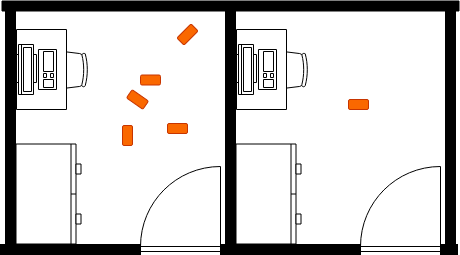
\includegraphics[width=\linewidth]{WrongLocalization}
  \caption{A boat.}
  \label{fig:boat1}
\end{figure}

The chances of wrong localization increases further when all robots try to localize within the limited space of received base map. As the number of localizing robots increases, the scene become more dynamic and it becomes difficult for a robot to localize. Also dynamic environment increases the probability of wrong localization.\par 
One way to solve this problem is to localize one robot at a time. So,even if all the robots are present in the base map, as they are not moving, the environment still remain static and localization become safer and faster. But localizing one robot at a time increases the time before the system attains its full potential. Also by the time the last robot completes localization, the base map would have developed significantly. So the time taken for the last robot to travel to next un-mapped area also adds to the time cost.

After a successful localization, we get the link between the local map and the global map.i.e. The transformation between global map and local map. This transformation is applied to every map updates in local map frame of reference and added to global map. The key factor in this process is getting the transformation. That is the reason why we require localization.\par
But if the transformation is already known, i.e. we know the link between global map and local map, the entire process becomes much simple and more resistant to failure. We acquire this by starting every robots at predetermined poses(position and orientation). We upload the robot id's and their poses in server before initializing the mapping process. Server computes the transformation between each robots and store it as initial static transformations. Using this transformation table, server can easily transform incoming map updates to global map.\par 
This solution for localizing problem can be easily implemented in simulations as all we have to do is spawn the robots at the predetermined poses and upload the data into the server. But it is extremely tough to attain in real life tasks. The global map depends heavily on the accuracy of initial transformations. If we fail to position the robot exactly the way we intended to, The global map can become unreliable. This error will be on top the inherent errors associated with SLAM such as drift etc.\par
There is a way to solve the problem without the need of (explicit)transformation at all.

\section{Image based Mapping Strategy}
In this strategy, we are eliminating the need for localization by making use of image aspects of map for stitching each map together. In this we are never making use of the transformation between robots. for this same reason, we do not need to start all robot in the mapping range of the robot which produces the initial map.\par
There should be enough overlap between maps for stitching them together. The steps of image stitching using a pair of images are given below
\begin{itemize}
    \item Identify Key-points in both the maps along with its descriptors. Descriptors are useful in identifying key-points from different images. If there are many elements in the map, many key-points can be identified.
    \item Comparing and Matching the key points. Cycling through the key-points and matching the similar points. This may include several outliers. Which are wrongly matched points.
    \item Filtering outliers. Finding out the matches which varies significantly from others.
    \itme Calculating the homography transformation between the maps from the inlier matches. We need at least 8 correct matches to calculate the homography matrix. This transformation defines how one map can be pasted over the other map.
    \item warp one map according to the homography transformation.
    \item Blend two maps together.
\end{itemize}

Key-points are considered as the point of interest in an image. They can be detected even if the image has undergone affine transformations. A keypoint and desctiptor defines a feature. In a map, more unique features gives better key-points and thus more reliable matches. This algorithm will work better when the environment has more edges, corners etc. 

A pseudo code for Image based Centralized MR SLAM is given below
\begin{algorithm}
 \caption{Image Based Centralized MR SLAM}\label{algorithm1}
%  \KwIn{this text}
%  \KwOut{how to write algorithm with \LaTeX2e }
 
 \textit{robot} initializes SLAM\;
 
 \While{biggest map on server has frontiers}{
 
  \textit{robot} perform SLAM and records local map\;
  
  \textit{robot} transmit local map to server\;
  
  \textit{server} receives local map from all robots\;
  
  \If{maps have sufficient overlap information between them}{
   
  \textit{server} generate a map stitching the map which has overlap\;
  
  
  \textit{server} updates both local map to the stitched map\;
  
  \textit{server} transmit the updated local map to the respective robots\;
   
   }
  \textit{robot} receives updated map\;
  
 }
 \textit{server} terminates mapping\;
 
\end{algorithm}

Although this strategy can be faster because we are skipping the need of localization, there are some drawbacks for this approach as well.
\begin{enumerate}
    \item We need map overlap for the algorithm to work. When the mapping is completed, there will be maps which has common regions. The size of this common region will depend on the environment type and how much information is available to make a successful stitch. The common areas implies that the same area has been mapped multiple times. This increases the time cost of scanning that region and also opportunity cost associated with repeating of information.
    \item Two robots being in communication range does not guarantee map merger. The maps should have enough overlapping information for the merger. 
    \item same area can get mapped more than once. This may cause discrepancies in the final merged map.
    \item This approach fails in a dynamic environment. As the process is not continuously adding features to a global map but merging parts of map together, it can fail to merge under dynamic environment. Since there can be differences in the map, the confidence factor has to be set lower which increases the chance of wrong map getting merged.
    \item Server has to manage many map fragments before it can merge them together. Causes more memory usage.
\end{enumerate}

As compared to Localization based approach, this approach do not need explicit time to calculate the transformations between robots through localization. It can start the mapping process right away and homography transformation becomes known as the mapping process goes on. Once a homography is found out between two map fragments from different robots, their subsequent map updates can be directly applied. \par
Since the robot starting within each one's mapping range is no longer needed, robots can be distributed strategically in the map so that they travel less distance and meet together in one common region which completes the map. Robot's initial position can affect the performance in this approach.\par 
The algorithm has a closed loop at the robot's end. i.e. Robots do not require server's intervention for them to perform mapping. Server does makes it easier and faster for robots to execute the task. So the robots can continue mapping without checking for server transmitted data. As soon as a merger is found, server updates the corresponding robots map.\par
So, This method uses a parallel architecture between robot and server as compared to serial architecture in the localization based approach.\par

\section{Simulation and Analysis}

Simulations are carried out using ROS. we use stage to simulate the environment and the robots. Maps are monitored in RVIZ. Navigation2D package is used for other robot functions such as navigation, obstacle avoidance, SLAM, etc. Google cartographer is the SLAM package used in the simulations.

\subsection{Localization Based Centralized SLAM}
For the localization based approach, the steps are as follows,
\begin{enumerate}
    \item Launch ROS packages for the simulation. important packages are robot packages, stage simulator and Rviz. 
    \item Load the environment in stage and spawn the robots at the predefined locations.
    \item Start initial mapping sequence for the first robot. This is a sequence of movements, going straight and then taking a complete rotation.
    \item The initial map is synced to the other robots through the server. This will be considered as a base for global map.
    \item Once other robots receive predefined area of map, A particle filter is initialized for localization.
    \item Localizing is performed with the particle filter. Particle filter is initialized within the received map at that specific instant. If the robot is outside the received map at that instant, the localizing will fail. This is why the assumption of every robot starts within the mapping are of every other robots very important.
    \item 
\end{enumerate}

\subsection{Image Based Centralized SLAM}

\subsection{Analysis}
 
\chapter{DECENTRALIZED MR-SLAM}
\label{chap:intro}
Unlike a centralized multi-robot system, a decentralized multi robot system lacks the presence of a central entity to control robots and manage the information collected by them. In a decentralized system, each robots will be independent, autonomous and able to process the information they collect. Also there is a limit to their communication range.
In a decentralized system, only local communication is possible. Two robots can communicate only if they are within the communication range of each other. Robots perform independent SLAM if they are not communicating. Each robot is perfectly capable of generating the map and finish the task all by themselves. Communication lets them share the map in between so that the process become faster. While performing SLAM, every robot will be checking if it can communicate to other robots. Once the robot finds one, the SLAM process is paused, and map information is shared between them. After processing the received information, both robots can continue their individual SLAM.
\section{Moving on from centralized strategy}
A centralized strategy cannot be applied to a decentralized system mainly because of,
\begin{enumerate}
    \item The robots are not in constant communication with other robots. Only possible mode of communication is local communication.
    \item The robots do not need to start within the mapping range of all other robots. They can start anywhere.
    \item Localizing one robot in the other robot's map will take significant amount of time considering the fact that number of such localization will be much higher than the centralized counterpart.
\end{enumerate}

\section{Mapping Strategy}
\section{Analysis}

\chapter{RandEx ALGORITHM}
\chapter{CONCLUSIONS AND RESULTS}
\label{chap:intro}

This document provides a simple template of how the provided
\verb+iitmdiss.cls+ \LaTeX\ class is to be used.  Also provided are
several useful tips to do various things that might be of use when you
write your thesis.

Before reading any further please note that you are strongly advised
against changing any of the formatting options used in the class
provided in this directory, unless you are absolutely sure that it
does not violate the IITM formatting guidelines.  \emph{Please do not
  change the margins or the spacing.}  If you do change the formatting
you are on your own (don't blame me if you need to reprint your entire
thesis).  In the case that you do change the formatting despite these
warnings, the least I ask is that you do not redistribute your style
files to your friends (or enemies).

It is also a good idea to take a quick look at the formatting
guidelines.  Your office or advisor should have a copy.  If they
don't, pester them, they really should have the formatting guidelines
readily available somewhere.

To compile your sources run the following from the command line:
\begin{verbatim}
% latex thesis.tex
% bibtex thesis
% latex thesis.tex
% latex thesis.tex
\end{verbatim}
Modify this suitably for your sources.

To generate PDF's with the links from the \verb+hyperref+ package use
the following command:
\begin{verbatim}
% dvipdfm -o thesis.pdf thesis.dvi
\end{verbatim}

\section{Package Options}

Use this thesis as a basic template to format your thesis.  The
\verb+iitmdiss+ class can be used by simply using something like this:
\begin{verbatim}
\documentclass[PhD]{iitmdiss}  
\end{verbatim}

To change the title page for different degrees just change the option
from \verb+PhD+ to one of \verb+MS+, \verb+MTech+ or \verb+BTech+.
The dual degree pages are not supported yet but should be quite easy
to add.  The title page formatting really depends on how large or
small your thesis title is.  Consequently it might require some hand
tuning.  Edit your version of \verb+iitmdiss.cls+ suitably to do this.
I recommend that this be done once your title is final.

To write a synopsis simply use the \verb+synopsis.tex+ file as a
simple template.  The synopsis option turns this on and can be used as
shown below.
\begin{verbatim}
\documentclass[PhD,synopsis]{iitmdiss}                                
\end{verbatim}

Once again the title page may require some small amount of fine
tuning.  This is again easily done by editing the class file.

This sample file uses the \verb+hyperref+ package that makes all
labels and references clickable in both the generated DVI and PDF
files.  These are very useful when reading the document online and do
not affect the output when the files are printed.


\section{Example Figures and tables}

Fig.~\ref{fig:iitm} shows a simple figure for illustration along with
a long caption.  The formatting of the caption text is automatically
single spaced and indented.  Table~\ref{tab:sample} shows a sample
table with the caption placed correctly.  The caption for this should
always be placed before the table as shown in the example.


\begin{figure}[htpb]
  \begin{center}
    \resizebox{50mm}{!} {\includegraphics *{iitm}}
    \resizebox{50mm}{!} {\includegraphics *{iitm}}
    \caption {Two IITM logos in a row.  This is also an
      illustration of a very long figure caption that wraps around two
      two lines.  Notice that the caption is single-spaced.}
  \label{fig:iitm}
  \end{center}
\end{figure}

\begin{table}[htbp]
  \caption{A sample table with a table caption placed
    appropriately. This caption is also very long and is
    single-spaced.  Also notice how the text is aligned.}
  \begin{center}
  \begin{tabular}[c]{|c|r|} \hline
    $x$ & $x^2$ \\ \hline
    1  &  1   \\
    2  &  4  \\
    3  &  9  \\
    4  &  16  \\
    5  &  25  \\
    6  &  36  \\
    7  &  49  \\
    8  &  64  \\ \hline
  \end{tabular}
  \label{tab:sample}
  \end{center}
\end{table}

\section{Bibliography with BIB\TeX}

I strongly recommend that you use BIB\TeX\ to automatically generate
your bibliography.  It makes managing your references much easier.  It
is an excellent way to organize your references and reuse them.  You
can use one set of entries for your references and cite them in your
thesis, papers and reports.  If you haven't used it anytime before
please invest some time learning how to use it.  

I've included a simple example BIB\TeX\ file along in this directory
called \verb+refs.bib+.  The \verb+iitmdiss.cls+ class package which
is used in this thesis and for the synopsis uses the \verb+natbib+
package to format the references along with a customized bibliography
style provided as the \verb+iitm.bst+ file in the directory containing
\verb+thesis.tex+.  Documentation for the \verb+natbib+ package should
be available in your distribution of \LaTeX.  Basically, to cite the
author along with the author name and year use \verb+\cite{key}+ where
\verb+key+ is the citation key for your bibliography entry.  You can
also use \verb+\citet{key}+ to get the same effect.  To make the
citation without the author name in the main text but inside the
parenthesis use \verb+\citep{key}+.  The following paragraph shows how
citations can be used in text effectively.

More information on BIB\TeX\ is available in the book by
\cite{lamport:86}.  There are many
references~\citep{lamport:86,prabhu:xx} that explain how to use
BIB\TeX.  Read the \verb+natbib+ package documentation for more
details on how to cite things differently.

Here are other references for example.  \citet{viz:mayavi} presents a
Python based visualization system called MayaVi in a conference paper.
\citet{pan:pr:flat-fst} illustrates a journal article with multiple
authors.  Python~\citep{py:python} is a programming language and is
cited here to show how to cite something that is best identified with
a URL.

\section{Other useful \LaTeX\ packages}

The following packages might be useful when writing your thesis.

\begin{itemize}  
\item It is very useful to include line numbers in your document.
  That way, it is very easy for people to suggest corrections to your
  text.  I recommend the use of the \texttt{lineno} package for this
  purpose.  This is not a standard package but can be obtained on the
  internet.  The directory containing this file should contain a
  lineno directory that includes the package along with documentation
  for it.

\item The \texttt{listings} package should be available with your
  distribution of \LaTeX.  This package is very useful when one needs
  to list source code or pseudo-code.

\item For special figure captions the \texttt{ccaption} package may be
  useful.  This is specially useful if one has a figure that spans
  more than two pages and you need to use the same figure number.

\item The notation page can be entered manually or automatically
  generated using the \texttt{nomencl} package.

\end{itemize}

More details on how to use these specific packages are available along
with the documentation of the respective packages.

%%%%%%%%%%%%%%%%%%%%%%%%%%%%%%%%%%%%%%%%%%%%%%%%%%%%%%%%%%%%
% Appendices.

\appendix

\chapter{A SAMPLE APPENDIX}

Just put in text as you would into any chapter with sections and
whatnot.  Thats the end of it.

%%%%%%%%%%%%%%%%%%%%%%%%%%%%%%%%%%%%%%%%%%%%%%%%%%%%%%%%%%%%
% Bibliography.

\begin{singlespace}
  \bibliography{refs}
\end{singlespace}


%%%%%%%%%%%%%%%%%%%%%%%%%%%%%%%%%%%%%%%%%%%%%%%%%%%%%%%%%%%%
% List of papers

\listofpapers

\begin{enumerate}  
\item Authors....  \newblock
 Title...
  \newblock {\em Journal}, Volume,
  Page, (year).
\end{enumerate}  

\end{document}